%!TEX root=../sub_lipsum.tex

% recognized by most of the editors


\section{Van der Waals Materials and the Two-Dimensional Crystal Revolution}
\label{sec:vdW_materials}

The isolation of atomically thin crystals from their layered bulk counterparts opened a new era in condensed matter physics.
Before this breakthrough, it was widely believed that strictly two-dimensional crystals could not exist in a thermodynamically stable free-standing form due to the divergence of long-wavelength thermal fluctuations in 2D~\cite{peierls-1935,mermin-1968}.
This view was overturned in 2004 when Novoselov, Geim, and co-workers demonstrated the isolation of graphene---a single monolayer of carbon atoms---from graphite using mechanical exfoliation~\cite{novoselov-2004}.
Their approach, colloquially known as the ``Scotch tape'' technique, proved that thermodynamically stable monolayer crystals could be fabricated and studied at room temperature.
The subsequent recognition that a broad family of layered van der Waals materials was amenable to the same approach triggered an explosion of interest in the so-called two-dimensional (2D) materials and their heterostructures~\cite{novoselov-2005}.

% \begin{figure}[H]
%     \centering
%     % \includegraphics[width=\textwidth]{Figure/Chapter_Lipsum/graphene_structure.png}
%     \caption{(a) Honeycomb lattice of graphene showing the two-sublattice (A, B) unit cell and the nearest-neighbour bond length $a_{CC} \approx 1.42$~\AA. (b) Electronic band structure of graphene; the linearly dispersing Dirac cones at the $K$ and $K'$ corners of the Brillouin zone give rise to massless Dirac fermions.}
%     \label{fig:graphene_structure}
%     % Source: Adapt from Novoselov et al. Science 306, 666 (2004) or Castro Neto et al. Rev. Mod. Phys. 81, 109 (2009).
% \end{figure}

\subsection{Graphene: The First Two-Dimensional Crystal}
\label{sec:graphene}

Graphene consists of a single layer of carbon atoms arranged in a two-dimensional honeycomb lattice.
Each carbon atom is $sp^2$-hybridised, forming three in-plane $\sigma$-bonds with its nearest neighbours at $120^\circ$ angles, while the remaining out-of-plane $p_z$ orbital contributes to a delocalised $\pi$-electron network.
The primitive unit cell contains two inequivalent carbon atoms (conventionally labelled A and B), forming two interpenetrating triangular sublattices.
The nearest-neighbour C-C bond length is $a_{CC} \approx 1.42$~\AA, giving an in-plane lattice constant $a = a_{CC}\sqrt{3} \approx 2.46$~\AA.

The electronic band structure of graphene features two inequivalent band-touching points at the $K$ and $K'$ corners of the hexagonal Brillouin zone---the so-called Dirac points.
Near these points, the energy dispersion is linear:
\begin{equation}
    E(\mathbf{k}) = \pm \hbar v_F |\mathbf{k}|,
    \label{eq:dirac_cone}
\end{equation}
where $v_F \approx 10^6$~m/s is the Fermi velocity.
The charge carriers therefore behave as massless Dirac fermions, making graphene a zero-gap semimetal with a vanishing density of states at the charge-neutrality (Dirac) point~\cite{novoselov-2004}.
This linear dispersion is the origin of graphene's celebrated properties: carrier mobilities exceeding $10^5$~cm$^2$V$^{-1}$s$^{-1}$ in suspended devices, a universal optical absorptance of $\pi\alpha \approx 2.3\%$ per layer (where $\alpha$ is the fine structure constant), and an ambipolar electric field effect tunable from $p$- to $n$-type by gating.

The absence of a bandgap, while fundamental to graphene's transport properties, limits its use as a semiconductor for optical emitters or transistors with high on/off ratios.
This limitation motivated the search for other 2D materials that preserve the advantages of the 2D geometry while adding a finite bandgap and richer internal degrees of freedom.

\subsection{The Family of Two-Dimensional Materials}
\label{sec:2D_family}

Beyond graphene, a large variety of layered materials can be mechanically exfoliated or grown by chemical vapour deposition (CVD) to yield monolayers and few-layer crystals spanning virtually the full range of electronic behaviour~\cite{novoselov-2005}:

\textit{Insulators.}
Hexagonal boron nitride (hBN) is a structural analogue of graphite in which the two honeycomb sublattices are occupied by boron and nitrogen atoms.
It has a wide indirect bandgap of approximately 6~eV, an atomically flat and chemically inert surface, and no dangling bonds.
Its in-plane lattice constant ($a \approx 2.50$~\AA) is close to that of graphene, making it an ideal substrate and encapsulant.

\textit{Semimetals.}
Graphene and bilayer graphene fall in this category, as do certain few-layer configurations of black phosphorus.

\textit{Semiconductors.}
The group-VI transition metal dichalcogenides---MoS$_2$, MoSe$_2$, WS$_2$, WSe$_2$---are the most intensively studied 2D semiconductors.
They undergo an indirect-to-direct bandgap transition upon thinning to the monolayer limit, yielding bright photoluminescence and rich excitonic physics.
They form the central subject of this thesis and are discussed in detail in Section~\ref{sec:TMDs}.

\textit{Metals and superconductors.}
NbSe$_2$ becomes superconducting below 7~K in bulk and retains superconductivity in the monolayer~\cite{novoselov-2005}.
Twisted bilayer graphene and moiré TMD heterostructures exhibit correlated insulating and superconducting phases at magic twist angles.

\textit{Magnets.}
CrI$_3$ and Cr$_2$Ge$_2$Te$_6$ are ferromagnetic insulators that preserve long-range magnetic order in the monolayer limit, opening routes to 2D spintronics.

The unifying feature of all these materials is that their bulk crystals are built from covalently bonded layers stacked by weak van der Waals forces.
Because no covalent bonds are broken upon exfoliation, individual monolayers are free of surface dangling bonds, and---crucially---different monolayers can be restacked in arbitrary sequences.

% \begin{figure}[H]
%     \centering
%     % \includegraphics[width=\textwidth]{Figure/Chapter_Lipsum/2D_material_family.png}
%     \caption{Overview of the 2D materials family, illustrating the range of electronic properties accessible: insulators (hBN), semimetals (graphene), semiconductors (TMDs), metals, superconductors, and magnets.}
%     \label{fig:2D_family}
%     % Source: Adapt from Novoselov et al. Science 353, aac9439 (2016), Fig. 1.
% \end{figure}

\subsection{Van der Waals Heterostructures and hBN Encapsulation}
\label{sec:hBN}

The concept of van der Waals heterostructures proposes to use the library of 2D monolayers as atomic-scale building blocks for designer materials assembled layer by layer~\cite{geim-2013}.
Since the layers interact only through weak van der Waals forces, different materials can be combined without the lattice-matching constraints that govern conventional semiconductor heteroepitaxy.
Each constituent layer can in principle retain its intrinsic electronic properties while acquiring new functionalities from proximity effects at the interfaces---electric gating, dielectric screening, moiré superlattice physics, and more.

For optical spectroscopy of TMDs, the most impactful heterostructure configuration is the hBN/TMD/hBN sandwich, in which the TMD monolayer is fully encapsulated between two thin hBN crystals.
The benefits of hBN encapsulation are multiple~\cite{cadiz-2017}:

\textit{Suppression of dielectric disorder.}
hBN presents an atomically flat surface free of dangling bonds and charged impurities.
When a TMD rests on amorphous SiO$_2$ instead, the electrostatic roughness of the oxide produces inhomogeneous spectral broadening that masks intrinsic optical features.
hBN encapsulation eliminates this extrinsic disorder.

\textit{Environmental protection.}
hBN's wide bandgap and chemical inertness shield the TMD from atmospheric adsorbates (water, oxygen) that dope the monolayer and quench emission.

\textit{Symmetric dielectric screening.}
The symmetric dielectric environment provided by top and bottom hBN modifies the Coulomb interaction within the TMD.
In particular, the non-local dielectric screening introduced by the hBN reduces excitonic binding energies by roughly a factor of two compared to a TMD on a bare SiO$_2$ substrate~\cite{raja-2017}.

\textit{Linewidth improvement.}
The net effect of encapsulation is a dramatic narrowing of optical resonances: in high-quality encapsulated WS$_2$ and WSe$_2$, the neutral exciton linewidth at low temperature can approach the homogeneous limit set by the radiative lifetime, and a rich zoo of excitonic complexes---trions, dark excitons, phonon replicas---becomes spectrally resolved~\cite{cadiz-2017,zinkiewicz-2021}.

% \begin{figure}[H]
%     \centering
%     % \includegraphics[width=\textwidth]{Figure/Chapter_Lipsum/hBN_encapsulation.png}
%     \caption{(a) Schematic of the hBN/WS$_2$/hBN encapsulated stack fabricated on a SiC membrane for Joule heating. (b) Comparison of low-temperature PL spectra for non-encapsulated (top) and encapsulated (bottom) WS$_2$ monolayers, illustrating the dramatic linewidth reduction achieved by hBN encapsulation.}
%     \label{fig:hBN_encap}
%     % Source: Panel (a) original schematic for this thesis; panel (b) adapted from Cadiz et al. PRX 7, 021026 (2017), or Zinkiewicz et al. Nano Lett. 21, 2175 (2021).
% \end{figure}


\section{Transition Metal Dichalcogenides}
\label{sec:TMDs}

\subsection{Crystal Structure}
\label{sub:chapKeyWord__subsection_2_1}

Transition metal dichalcogenides (TMDs) are layered compounds with the general formula MX$_2$, where M is a group-VI transition metal atom (Mo or W) and X is a chalcogen atom (S, Se, or Te).
As illustrated in Figure~\ref{fig:TMD}, the relevant elements are concentrated in specific rows of the periodic table.
Like graphite, bulk TMDs consist of a vertical stack of MX$_2$ trilayers weakly coupled by van der Waals interactions, making mechanical exfoliation to monolayers straightforward.

\begin{figure}[htbp]
	\centering
	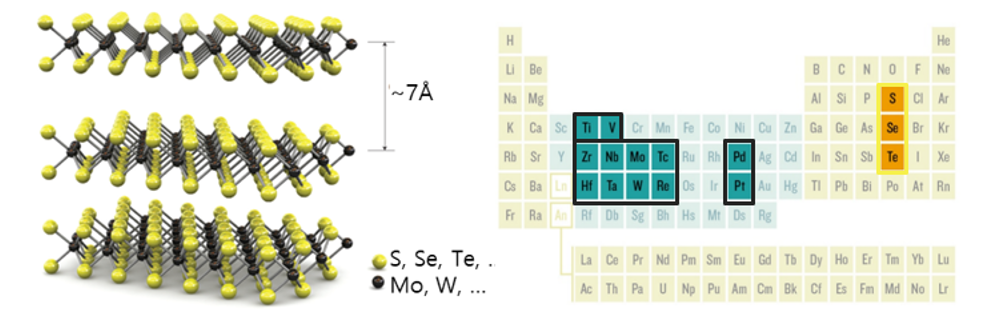
\includegraphics[width=\textwidth]{Figure/Chapter_Lipsum/TMD.png}
	\caption{(a) Layered crystal structure of a transition metal dichalcogenide, illustrating the X-M-X trilayer units stacked by van der Waals forces. (b) Relevant transition metal atoms (Mo, W; green) and chalcogen atoms (S, Se, Te; orange) in the periodic table.}
	\label{fig:TMD}
\end{figure}

The thermodynamically stable polymorph of the semiconducting TMDs studied in this work is the 2H (hexagonal) phase.
As shown in Figure~\ref{fig:TMD_2H}, the 2H structure features trigonal prismatic coordination of the metal atom: the two chalcogen planes are directly eclipsed in projection, and the unit cell contains one metal and two chalcogen atoms.
Viewed from above, the monolayer has a honeycomb-like appearance with alternating M and X$_2$ sites.
The in-plane lattice constant is $a \approx 3.15$~\AA\ for WS$_2$~\cite{fabian2022}.

\begin{figure}[htbp]
	\centering
	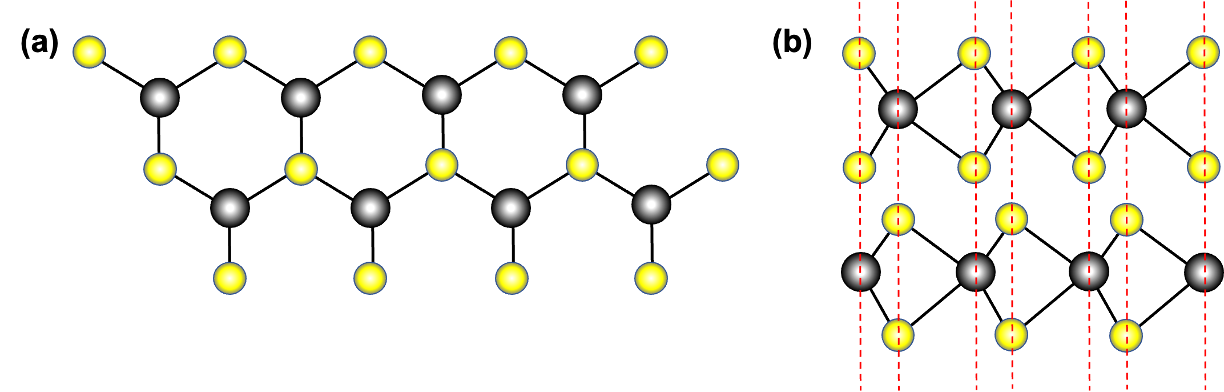
\includegraphics[width=\textwidth]{Figure/Chapter_Lipsum/TMD_2H.png}
	\caption{The 2H phase of a TMD monolayer. (a) Top view showing the hexagonal arrangement of metal (blue) and chalcogen (yellow) atoms. (b) Side view of the X-M-X trilayer with trigonal prismatic coordination. The 2H phase is the thermodynamically stable form for MoX$_2$ and WX$_2$ compounds.}
	\label{fig:TMD_2H}
\end{figure}

A critical structural feature of the 2H \textit{monolayer} is the breaking of inversion symmetry: unlike the bulk crystal (which is centrosymmetric because the two trilayers in its unit cell are related by inversion), the isolated monolayer lacks an inversion centre.
This broken inversion symmetry, combined with strong spin-orbit coupling from the heavy transition metal $d$ orbitals, has profound consequences for the electronic structure and optical selection rules discussed below.

\begin{figure}[htbp]
	\centering
	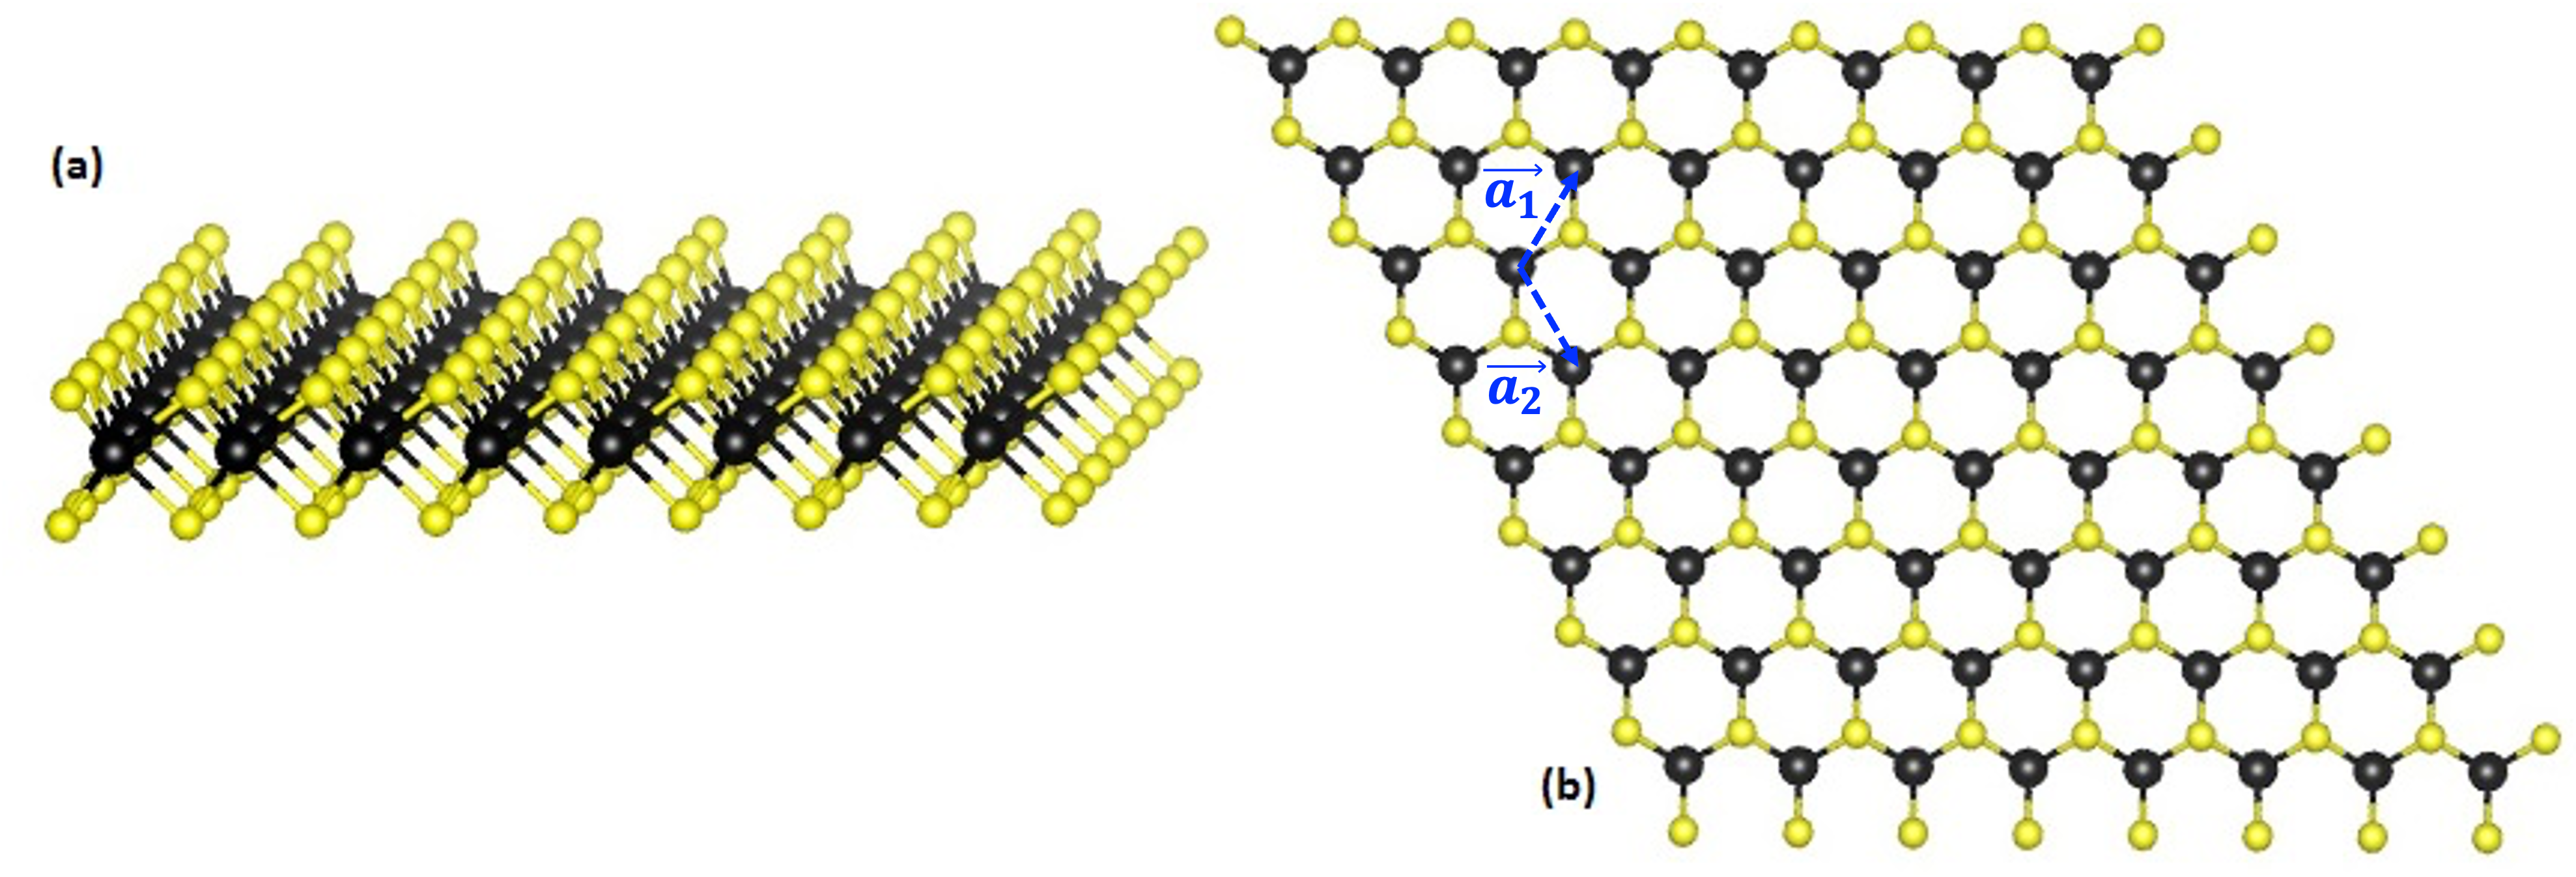
\includegraphics[width=\textwidth]{Figure/Chapter_Lipsum/TMD_2D.png}
	\caption{Structural representations of a monolayer TMD. (a) Three-dimensional representation showing the X-M-X sandwich. (b) Two-dimensional side view clarifying the in-plane covalent bonding (strong) and the interlayer van der Waals coupling (weak) in the bulk.}
	\label{fig:TMD_2D}
\end{figure}

As shown in Figure~\ref{fig:TMD_2D}, each monolayer is a covalently bonded X-M-X trilayer approximately 6~\AA\ thick.
The strong in-plane covalent bonds contrast with the much weaker interlayer van der Waals interaction, making it straightforward to isolate a monolayer from a bulk crystal by mechanical exfoliation.

\begin{figure}[htbp]
	\centering
	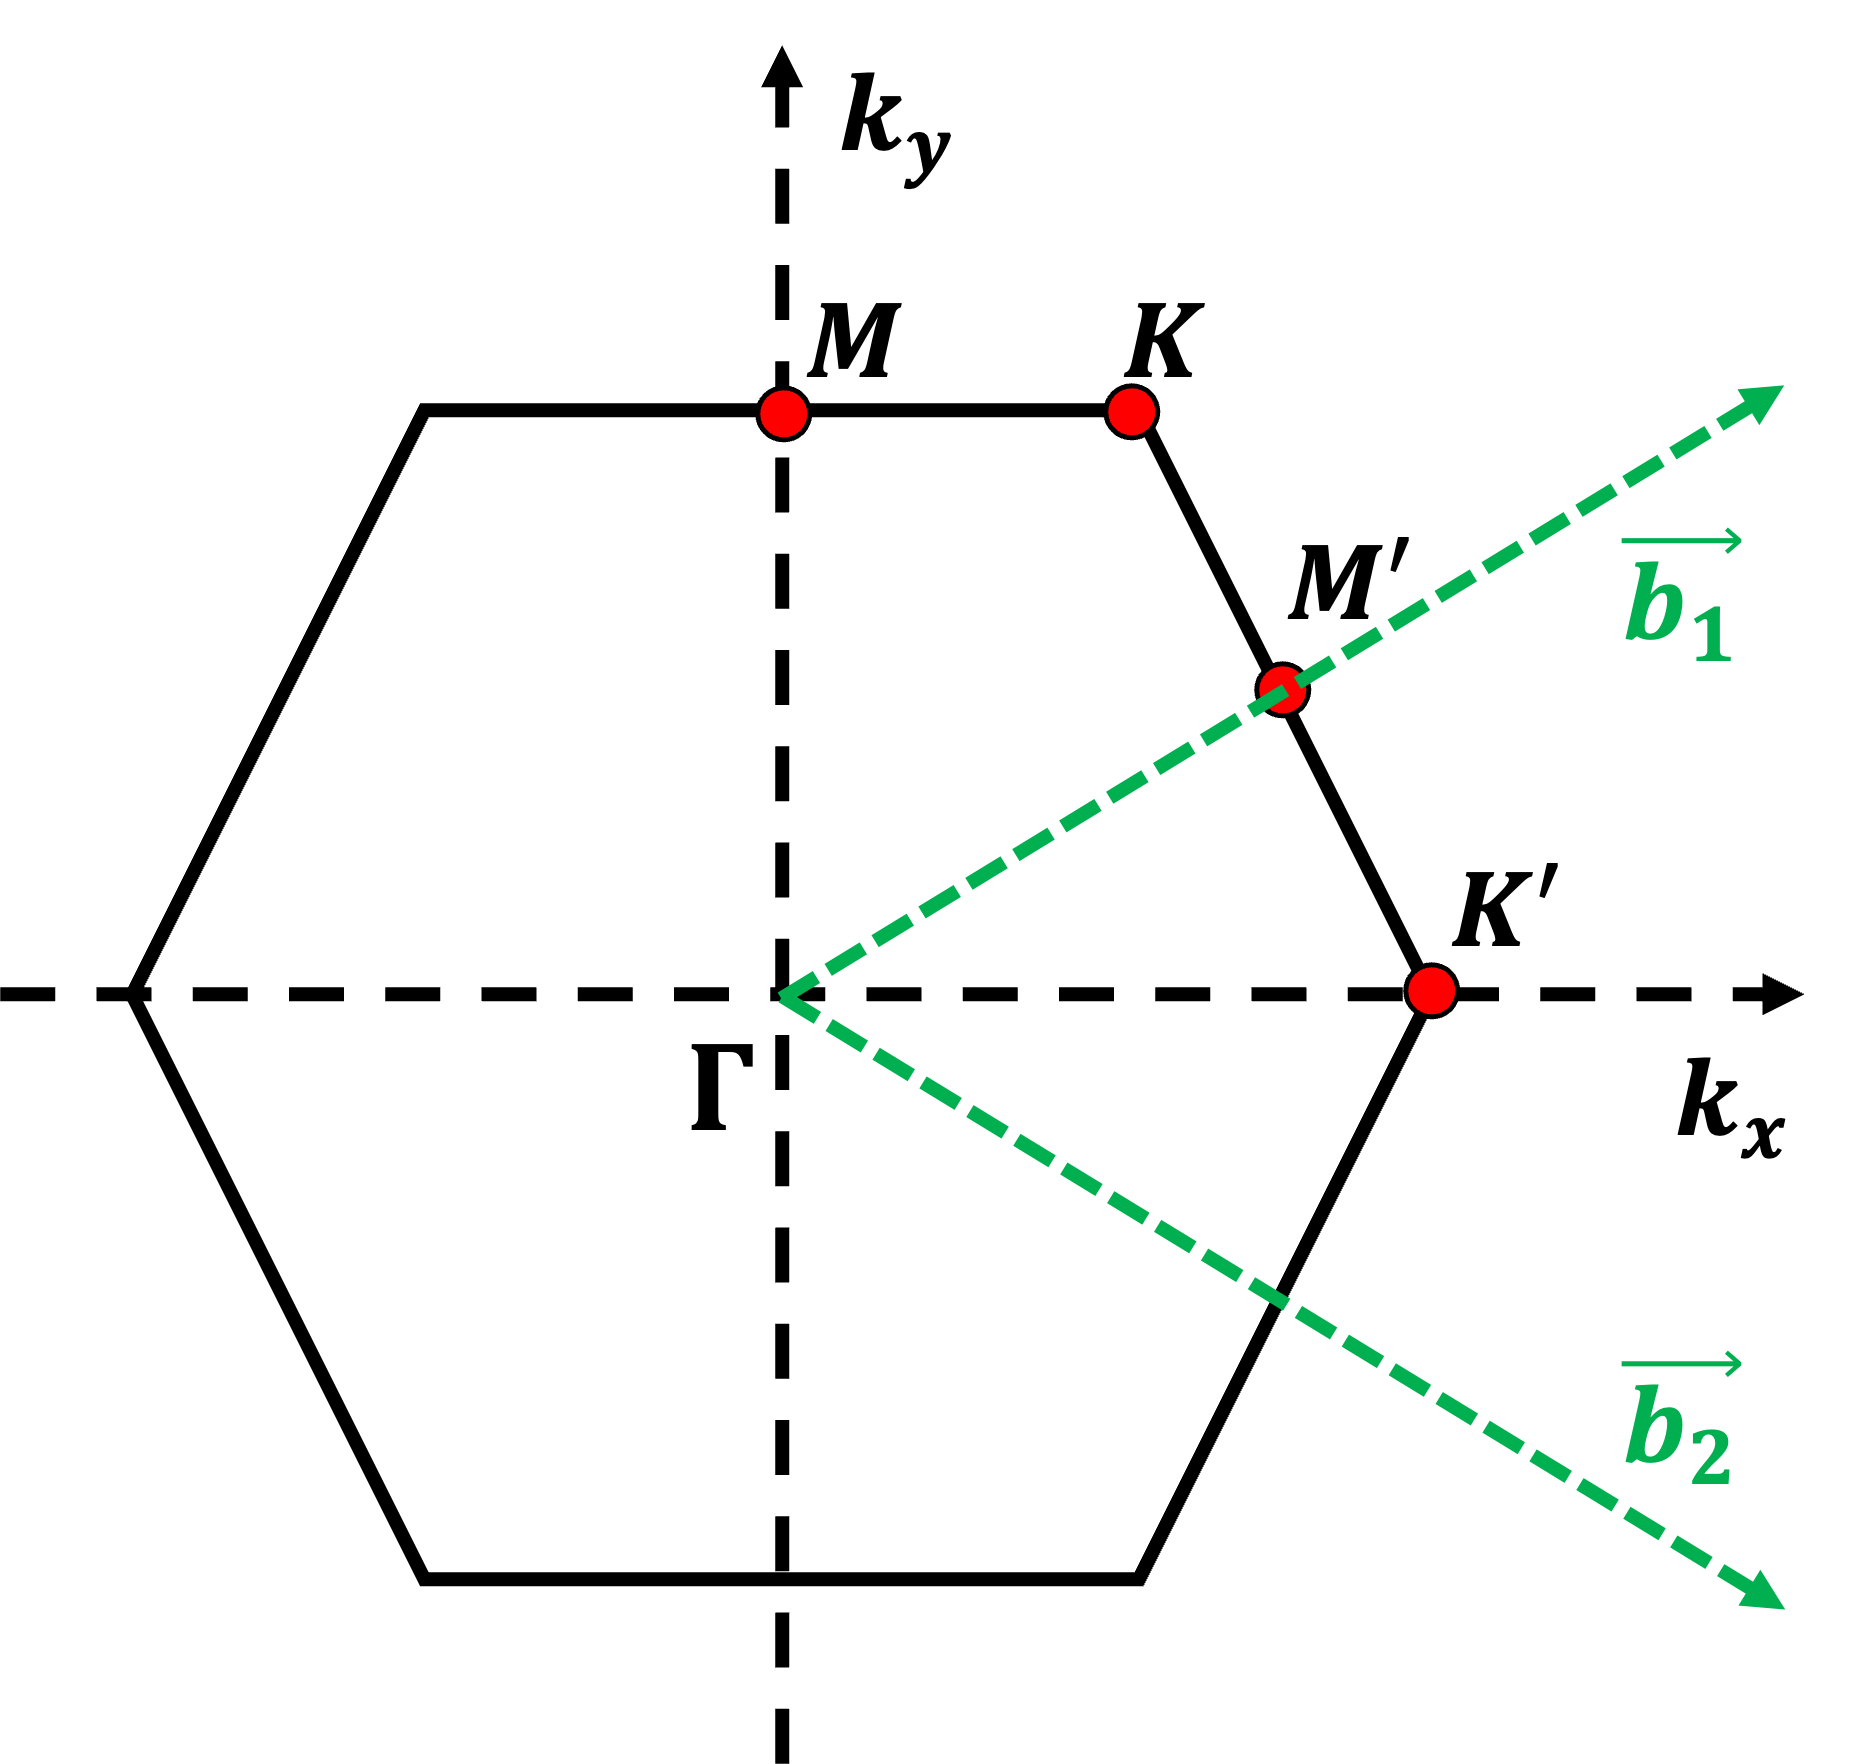
\includegraphics[width=0.5\textwidth]{Figure/Chapter_Lipsum/TMD_BZ.png}
	\caption{First Brillouin zone (BZ) of the hexagonal 2H-TMD lattice, with high-symmetry points $\Gamma$ (zone centre), $M$ (zone edge midpoints), $K$ and $K'$ (non-equivalent zone corners), and $\Lambda$ (midpoint of the $\Gamma$-$K$ line) labelled.}
	\label{fig:TMD_BZ}
\end{figure}

The hexagonal 2D Brillouin zone of the TMD monolayer is shown in Figure~\ref{fig:TMD_BZ}.
Its corners define the inequivalent $K$ and $K'$ points ($K' = -K$ under time reversal), which are the electronically most important high-symmetry points: in the monolayer limit they host both the valence band maximum and the conduction band minimum, making the bandgap direct~\cite{fabian2022}.

\subsection{Indirect-to-Direct Bandgap Transition}
\label{sub:chapKeyWord__subsection_2_bandgap}

In their bulk form, group-VI TMDs have an indirect bandgap between the valence band maximum near the $\Gamma$ point and the conduction band minimum at the $\Lambda$ point (midpoint of the $\Gamma$-$K$ line) or at $K$~\cite{fabian2022}.
As the crystal is thinned to a monolayer, a striking transformation occurs: the global bandgap becomes direct, with both the valence band maximum and the conduction band minimum located at the $K$ (and $K'$) corners of the hexagonal Brillouin zone.
This indirect-to-direct transition was first demonstrated experimentally in MoS$_2$ by Splendiani \textit{et al.}~\cite{splendiani-2010} and Mak \textit{et al.}~\cite{mak-2010}, who observed a dramatic enhancement---by orders of magnitude---of the photoluminescence quantum yield upon thinning to a single layer.
The same transition is well established in WS$_2$, MoSe$_2$, and WSe$_2$.

\begin{figure}[htbp]
    \centering
    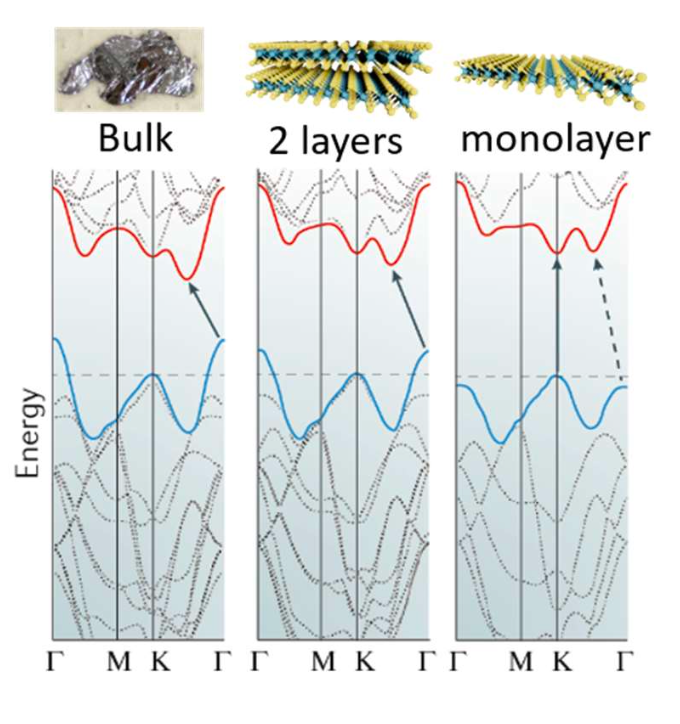
\includegraphics[width=0.7\textwidth]{Figure/Chapter_Lipsum/TMD_band.png}
    \caption{Calculated band structures of MoS$_2$ from bulk to monolayer~\cite{fabian2022}. In the bulk, the valence band maximum is at $\Gamma$ and the conduction band minimum is at $\Lambda$, giving an indirect gap. As the number of layers decreases, the $\Gamma$-valence and $\Lambda$-conduction band edges shift (dashed arrows in Fig.~\ref{fig:brightdark}) until the monolayer has a direct gap at $K$ (filled arrows). The solid arrows indicate the lowest energy transition in each case.}
    \label{fig:TMD_band}
\end{figure}

The physical origin of this transition can be understood from the orbital character of the band edges~\cite{fabian2022}.
The $K$-point valence and conduction band edges are formed predominantly by the metal $d_{x^2-y^2}$, $d_{xy}$ and $d_{z^2}$ orbitals, which are strongly localised within the metal plane and therefore relatively insensitive to interlayer coupling.
In contrast, the $\Gamma$-point valence band and the $\Lambda$-point conduction band have significant chalcogen $p_z$ character and interlayer hybridisation, making them strongly sensitive to layer number.
As the crystal is thinned, these interlayer-hybridised states shift rapidly in energy: the $\Gamma$ valence band moves down and the $\Lambda$ conduction band moves up, until in the monolayer the lowest-energy gap is the $K$-$K$ direct transition.

\subsection{Electronic Structure: Spin-Orbit Coupling and Valley Physics}
\label{sub:chapKeyWord__subsection_2_2}

\subsubsection{Spin-Orbit Splitting}

The heavy transition metals (Mo, W) introduce strong spin-orbit coupling (SOC) that, combined with the broken inversion symmetry of the monolayer, produces a large spin splitting of the band edges at $K$~\cite{kormanyos-2015}.
In WS$_2$, the valence band splitting $\Delta_\mathrm{VB} \approx 400$~meV and the conduction band splitting $\Delta_\mathrm{CB} \approx 30$~meV~\cite{kormanyos-2015}.
Time-reversal symmetry requires that the spin ordering at $K'$ is opposite to that at $K$: where $K$ has spin-up in the upper VB subband, $K'$ has spin-down (Figure~\ref{fig:brightdark}).

\subsubsection{Valley Degree of Freedom and Valley-Selective Optical Selection Rules}

The two inequivalent $K$ and $K'$ valleys, related by time reversal, constitute a binary pseudospin---the valley index~\cite{xiao-2012}.
Because the Berry curvature is equal and opposite at $K$ and $K'$, circularly polarised light couples selectively to each valley: $\sigma^+$ photons generate excitons in the $K$ valley, while $\sigma^-$ photons address the $K'$ valley~\cite{xiao-2012}.
This valley-selective circular dichroism, unique to the inversion-symmetry-broken monolayer, forms the basis of the emerging field of valleytronics.

Spin-valley locking further constrains the optical selection rules: because the spin orientation is locked to the valley index in the VB, the optical spin Hall effect and valley polarisation of the exciton emission are directly controlled by the helicity of the excitation laser.
Intervalley scattering, which requires a simultaneous change of both spin and valley, is strongly suppressed, enabling long-lived valley polarisation under resonant excitation.

Illustration of the spin-orbit split subbands is shown in Figure~\ref{fig:brightdark}.
The electronic band becomes spin-split and spin-polarised due to the broken inversion symmetry in the monolayer limit.
In monolayer WS$_2$, the transition between the uppermost valence band subband and the lowest conduction band subband is optically inactive due to spin conservation, as discussed in detail in Section~\ref{sec:brightdark_wse2}.

\begin{figure}[H]
    \centering
    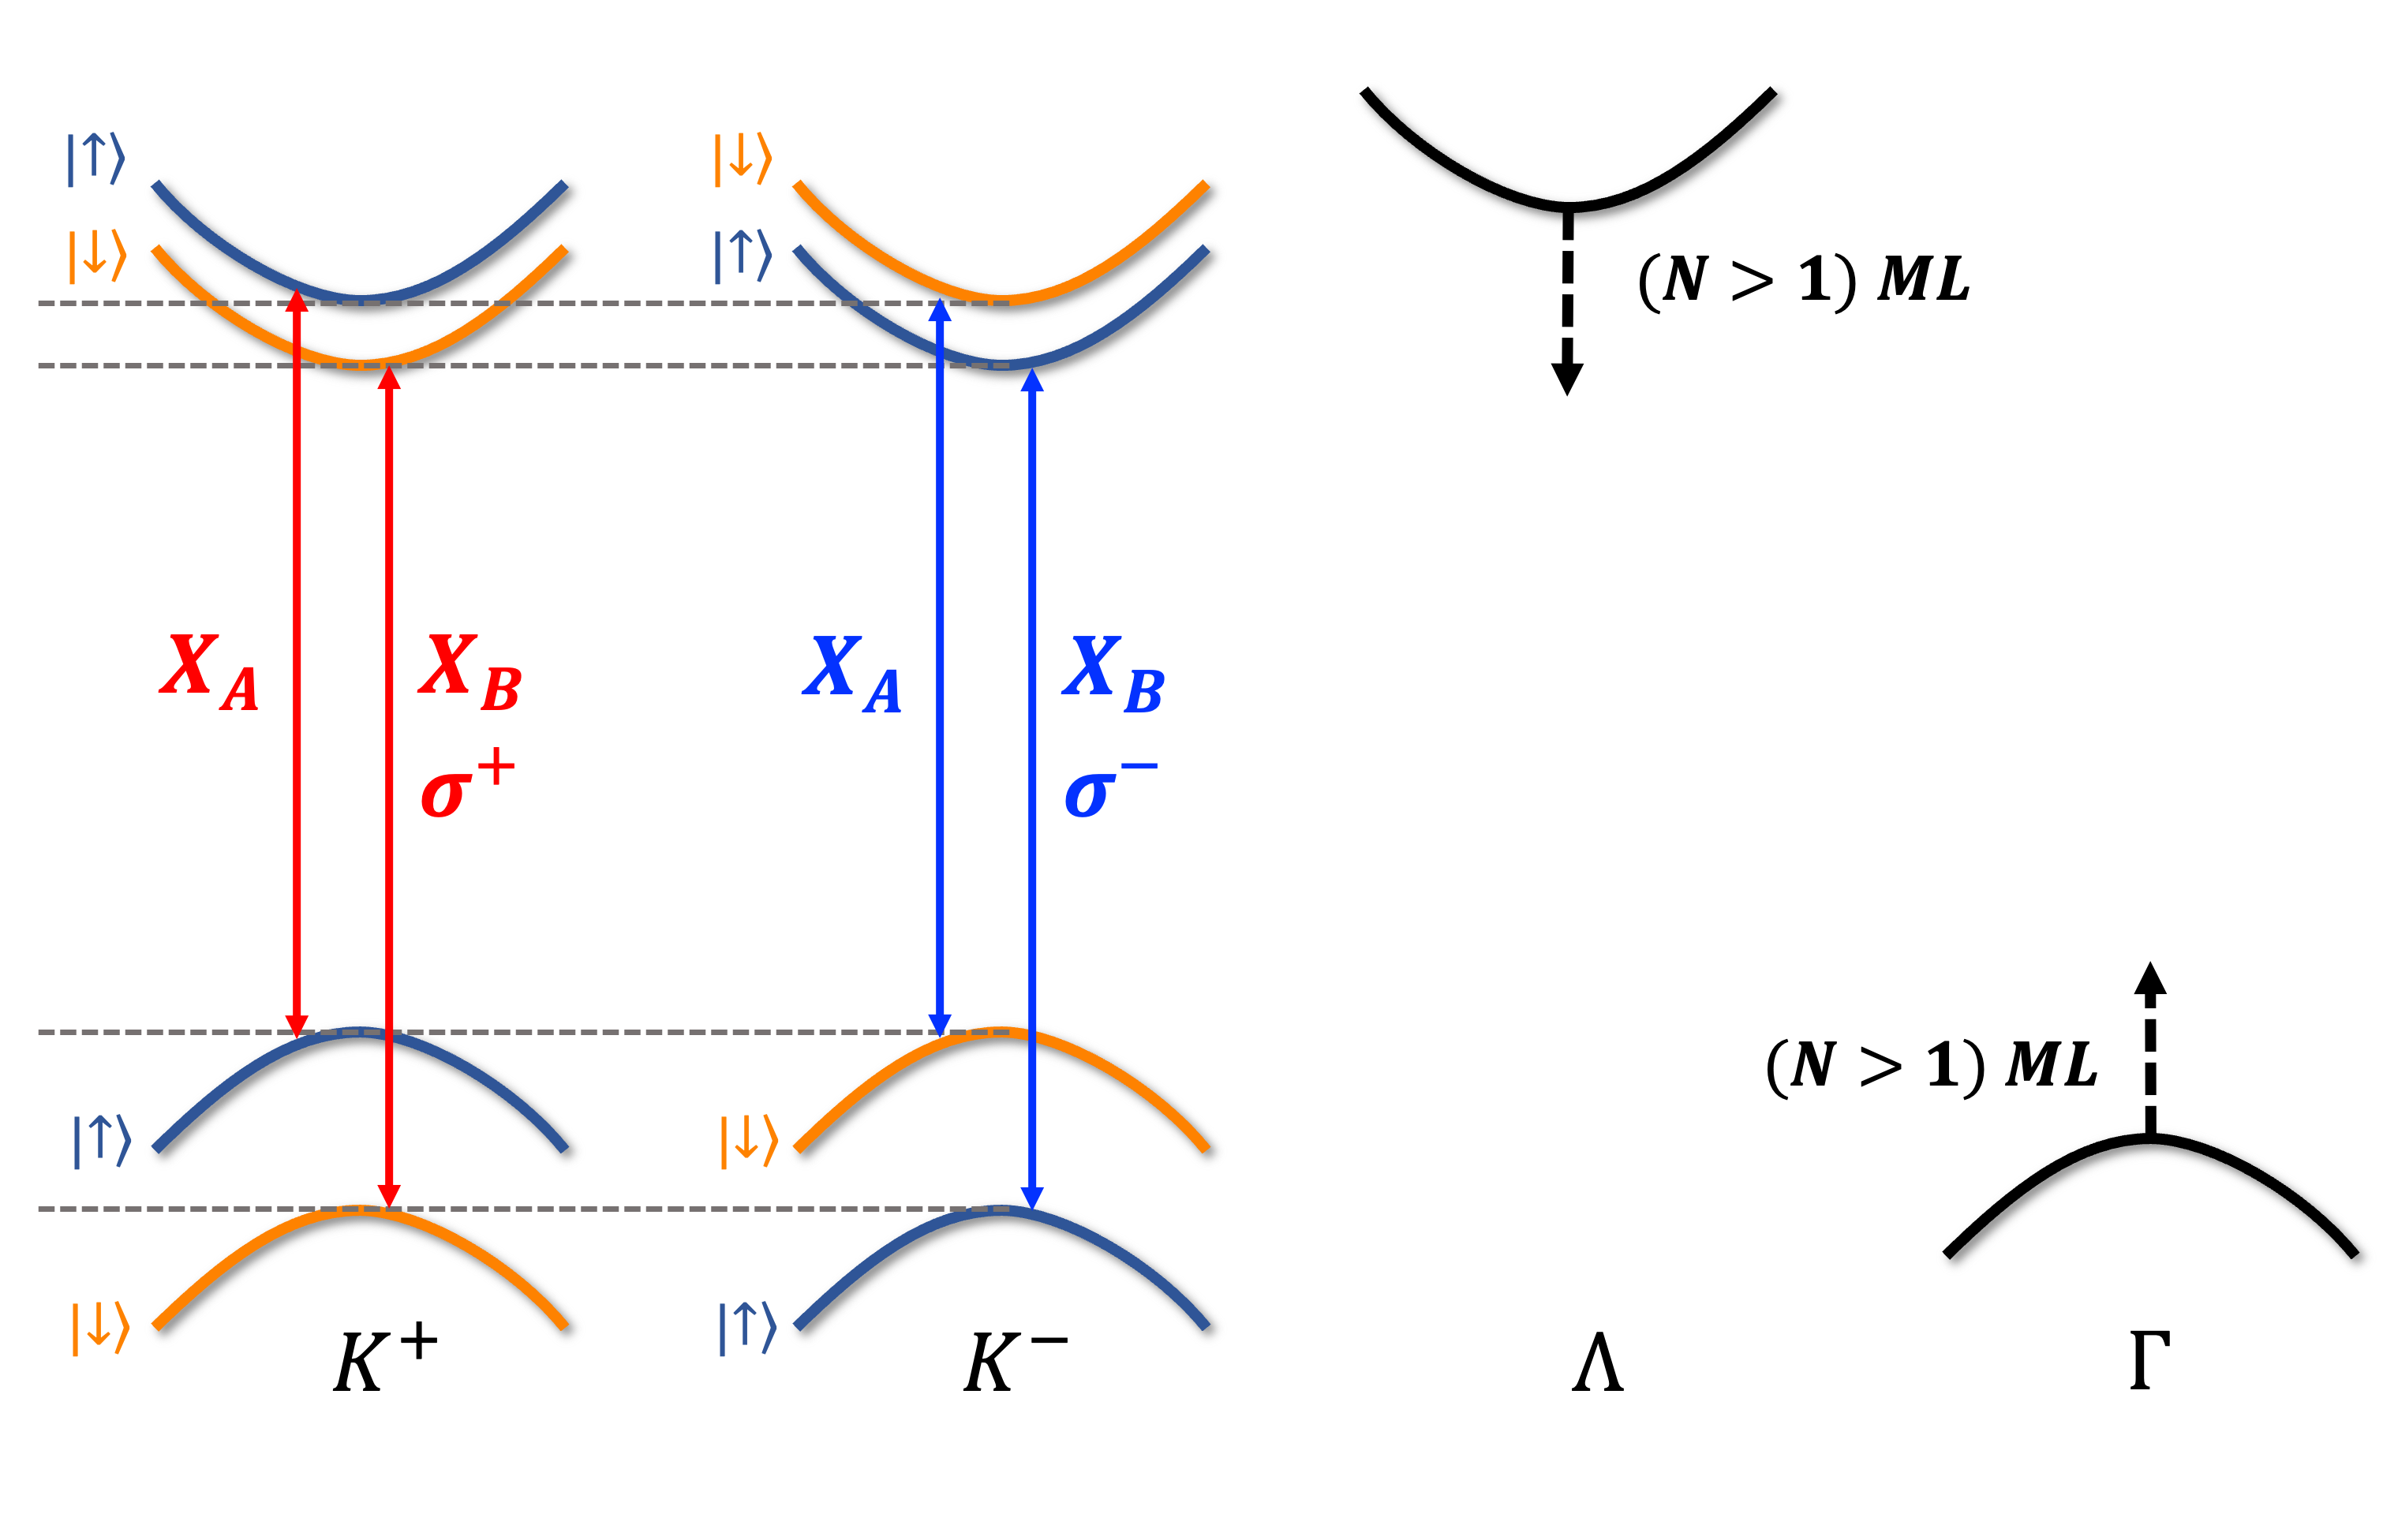
\includegraphics[width=\textwidth]{Figure/Chapter_Lipsum/brightdark.png}
    \caption{Diagram of the relevant conduction and valence band subbands at the $K^+$, $K^-$, and $\Lambda$ points of the Brillouin zone of monolayer WS$_2$. The arrows indicate the spin orientation (red = spin up, blue = spin down). The bright A-exciton ($X_A$) and B-exciton ($X_B$) transitions are shown; the dark A-exciton (momentum-forbidden transition between parallel-spin subbands) lies at lower energy due to the $\sim 30$~meV CB splitting. Black dashed arrows indicate the energy shifts of the $\Lambda$ (CB) and $\Gamma$ (VB) band edges upon increasing layer number, which convert the gap from direct (monolayer) to indirect (multilayer)~\cite{molas2017optical}.}
    \label{fig:brightdark}
\end{figure}

\subsection{Excitons in Two Dimensions}
\label{sub:chapKeyWord__subsection_2_4}

The optical response of monolayer TMDs is dominated by excitons: Coulomb-bound electron-hole pairs.
The strict two-dimensional confinement combined with significantly reduced dielectric screening makes excitonic effects in monolayer TMDs exceptionally strong.

\subsubsection{Non-Hydrogenic Exciton Rydberg Series and Binding Energy}

In a conventional three-dimensional semiconductor, the exciton follows a hydrogen-like Rydberg series $E_n = -E_0/n^2$ with principal quantum number $n = 1, 2, 3, \ldots$.
In two dimensions, the classical 2D Rydberg series is modified to $(n-\tfrac{1}{2})^{-2}$ and the binding energy is fourfold larger than in 3D; but in real TMD monolayers the situation is further complicated by the non-local dielectric screening of the 2D crystal~\cite{chernikov-2014}.
The dielectric function of a thin polarisable sheet embedded between two semi-infinite dielectric media is strongly momentum-dependent: at small in-plane wavevectors $q \ll r_0^{-1}$ (where $r_0$ is the screening length characterising the TMD polarisability) the screening is greatly reduced, and the Coulomb interaction deviates substantially from the bare $1/r$ form~\cite{chernikov-2014}.
This leads to a non-hydrogenic exciton Rydberg series in which the energy spacings between successive $ns$ states are compressed relative to the hydrogen atom, as confirmed by linear optical spectroscopy~\cite{chernikov-2014}.

Experimentally, exciton binding energies of order 300--500~meV have been measured in monolayer MoS$_2$, WS$_2$, and WSe$_2$~\cite{chernikov-2014}, compared to typical values of a few meV in bulk GaAs.
The corresponding exciton Bohr radius is $a_X \sim 1$--2~nm, making 2D excitons essentially point-like on the scale of optical wavelengths.
The large binding energy---far exceeding room-temperature thermal energy ($k_BT \approx 25$~meV at 300~K)---means that excitons are stable and dominate the optical response even at room temperature.

The strong sensitivity of the exciton binding energy to the dielectric environment is captured by the theory of non-local dielectric screening~\cite{raja-2017}: the exciton binding energy decreases as the average dielectric constant of the surrounding media increases.
This explains why hBN encapsulation reduces the binding energy by roughly a factor of two relative to a TMD on SiO$_2$ (see Section~\ref{sec:hBN}).

\subsubsection{Excitonic Complexes: Trions and Beyond}

In addition to the neutral exciton $X^0$, several multi-particle complexes are routinely observed in doped TMD monolayers.
Trions ($X^\pm$) are charged excitons formed by binding an extra electron ($X^-$) or hole ($X^+$) to the neutral exciton.
In TMDs, spin-valley locking generates two distinct negative trion states: the intervalley triplet trion $T^T$ (electrons in opposite valleys, spin triplet) and the intravalley singlet trion $T^S$ (both electrons in the same valley, spin singlet)~\cite{zinkiewicz-2021}.
Their binding energies differ slightly and the two peaks can be resolved in high-quality encapsulated samples.
Trion binding energies in WS$_2$ are typically 20--30~meV.

At higher excitation densities, biexciton ($XX$) states bound by two excitons can be observed, with binding energies of order 5--20~meV.
In TMD heterostructures, spatially indirect interlayer excitons form when the electron and hole reside in different TMD layers; these have long radiative lifetimes and a permanent dipole moment, making them attractive for dipolar quantum simulation.

\subsection{Bright and Dark Excitonic States in WS$_2$}
\label{sec:brightdark_wse2}

A defining feature of monolayer WS$_2$ (and its sister material WSe$_2$) is the \textit{darkish} character of its excitonic ground state~\cite{molas2017optical}.
As shown in Figure~\ref{fig:brightdark}, the conduction band at $K$ is spin-split by $\Delta_\mathrm{CB} \approx 30$~meV.
The upper CB subband ($\uparrow$ at $K$, $\downarrow$ at $K'$) is anti-parallel to the upper VB subband spin, making the $K^\uparrow$-CB to $K^\uparrow$-VB transition spin-conserving and optically bright (the bright A-exciton $X_A$).
The lower CB subband ($\downarrow$ at $K$, $\uparrow$ at $K'$) is parallel to the upper VB subband spin: the corresponding transition is spin-forbidden and optically dark (the dark A-exciton $X_A^D$).

Crucially, in WS$_2$ the CB splitting places the dark state \textit{below} the bright state in energy by $\sim$30~meV~\cite{kormanyos-2015}.
This is the opposite of so-called ``bright'' materials such as MoSe$_2$ and MoTe$_2$, in which the CB spin ordering is reversed and the bright exciton is the ground state.

The darkish character of WS$_2$ has far-reaching consequences for its low-temperature PL.
As shown in Figure~\ref{fig:darkpl}(a), the non-encapsulated WS$_2$ PL spectrum at 5~K is dominated by a forest of peaks below the bright exciton resonance~\cite{molas2017optical}.
These peaks arise from the multitude of recombination channels unlocked by the low-lying dark exciton: phonon-assisted recombination (phonon sidebands of dark trions), impurity-bound excitons, donor-acceptor pair recombination, and localised exciton emission.
The peaks $L_1$--$L_4$ are tentatively associated with localised or bound excitons; $T_2$ is likely an impurity-bound charged exciton.
The overall spectrum of non-encapsulated samples is notoriously sample-dependent and difficult to reproduce, reflecting its sensitivity to the specific disorder landscape of each flake.

In hBN-encapsulated WS$_2$, the suppression of dielectric disorder and the symmetric electrostatic environment allow the intrinsic excitonic species to be individually resolved~\cite{zinkiewicz-2021}.
As shown in Figure~\ref{fig:darkpl}(b), the encapsulated PL spectrum at low temperature reveals: the bright neutral exciton ($X_A^B$), the triplet negative trion ($T^T$) and singlet negative trion ($T^S$), the neutral dark exciton ($X_A^D$, which becomes visible by coupling to out-of-plane polarised light collected with a high-NA objective), multiple dark trion states, and their phonon replicas.
This rich excitonic fingerprint serves as the reference against which defect-related emission is identified in subsequent chapters.

\begin{figure}[H]
    \centering
    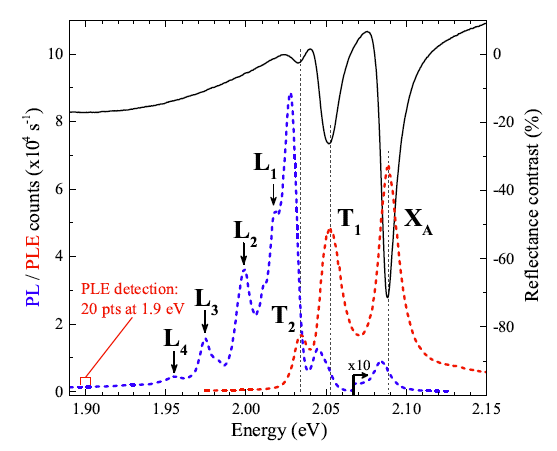
\includegraphics[width=\textwidth]{Figure/Chapter_Lipsum/darkpl.png}
    \caption{(a) Low-temperature ($\sim 5$~K) optical spectra of a non-encapsulated WS$_2$ monolayer: photoluminescence (PL, blue dashed), photoluminescence excitation (PLE, red dashed), and reflectance contrast (RC, black solid)~\cite{molas2017optical}.
    The RC shows two main resonances (neutral exciton $X_A$ and charged exciton $T_1$), while the PL is dominated by many additional peaks below these resonances, originating from dark and localised excitonic states.
    (b) Low-temperature PL spectrum of an $n$-doped hBN-encapsulated WS$_2$ monolayer at zero and in-plane magnetic field ($B_\parallel = 10$~T)~\cite{zinkiewicz-2021}, resolving the bright exciton ($X_B$), triplet and singlet trions ($T^T$, $T^S$), dark neutral exciton ($X_D$), dark trions, and their phonon replicas.}
    \label{fig:darkpl}
\end{figure}


\section{Atomic Defects and Single-Photon Emitters in TMDs}
\label{sec:defects_SPE}

\subsection{Point Defects in Monolayer TMDs}
\label{sub:chapKeyWord__subsection_3_1}

Real TMD crystals inevitably harbour point defects---local departures from perfect periodicity.
Among the native defects in MoX$_2$ and WX$_2$ compounds, chalcogen vacancies (V$_X$: a missing chalcogen atom on the upper or lower chalcogen plane) have the lowest formation energy and are the dominant intrinsic defect in both as-grown and annealed samples~\cite{komsa-2015}.
Other native defects include metal vacancies (V$_M$), antisite defects (a chalcogen atom on a metal site, or \textit{vice versa}), chalcogen adatoms, and substitutional impurities.
Density functional theory (DFT) calculations show that a single sulfur vacancy in MoS$_2$ or WS$_2$ introduces several in-gap electronic states whose energy and occupation depend on the charge state of the vacancy (neutral V$_S^0$, singly charged V$_S^+$, \textit{etc.})~\cite{komsa-2015}.

Several experimental routes exist for controlled defect engineering:

\textit{He$^+$ ion irradiation.}
A helium ion microscope (HIM) focuses a beam of He$^+$ ions to a sub-nanometre spot, creating chalcogen vacancies at a controlled dose and position~\cite{barthelmi2020atomistic}.
This technique offers the best spatial resolution but risks cumulative radiation damage at high doses.

\textit{Electron beam irradiation.}
In a scanning transmission electron microscope (STEM), the focused electron beam can displace individual chalcogen atoms with atomic precision, allowing real-time imaging and deliberate manipulation of single vacancies~\cite{noh-2014}.

\textit{Plasma treatment.}
Oxygen, argon, or sulfur-fluoride plasmas provide a chemical route to vacancy creation over macroscopic areas; the defect density is controlled by exposure time and power.

\textit{Thermal annealing.}
At temperatures above a material-dependent threshold, thermally activated bond breaking and chalcogen desorption generate vacancies in a dose controlled by temperature and dwell time~\cite{mitterreiter2021role}.
This approach avoids in-beam damage and can be performed in situ, making it particularly attractive for studying the relationship between vacancy density and optical properties.
The thermal annealing strategy forms the basis of the experimental work presented in this thesis.

% \begin{figure}[H]
%     \centering
%     % \includegraphics[width=\textwidth]{Figure/Chapter_Lipsum/defect_methods.png}
%     \caption{Methods for controlled generation of chalcogen vacancies in monolayer TMDs: (a) focused He-ion irradiation; (b) STEM electron beam; (c) plasma treatment; (d) thermal annealing. Each technique offers different spatial resolution, dose control, and lattice damage characteristics.}
%     \label{fig:defect_methods}
%     % Source: adapted for this thesis. Panel (a): Barthelmi et al. APL Mater. 8, 011007 (2020). Panel (d): Mitterreiter et al. Nat. Commun. 12, 3822 (2021).
% \end{figure}

\subsection{The Role of Chalcogen Vacancies}
\label{sub:chapKeyWord__subsection_3_2}

\begin{figure}[htbp]
    \centering
    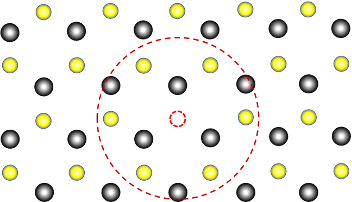
\includegraphics[width=0.6\textwidth]{Figure/Chapter_Lipsum/vacancy.png}
    \caption{Chalcogen vacancy defect in a TMD monolayer. The red dotted circle indicates the exciton Bohr radius ($a_X \sim 2$--3~nm), which is comparable to the inter-vacancy spacing at experimentally relevant densities, ensuring that individual vacancies act as isolated trapping centres for diffusing excitons.}
    \label{fig:vacancy}
    % Source: Figure/Chapter_Lipsum/vacancy.png
    % --> Copy from /tex file/CSI 1st/images/vacancy.png to Figure/Chapter_Lipsum/
\end{figure}

In semiconductors, free excitons interact with the Coulomb potential of lattice defects and can become localised as defect-bound exciton complexes.
The localisation introduces an additional binding energy relative to the free exciton, so that photon emission from defect-bound excitons appears red-shifted below the free exciton resonance.
In 2D TMDs, two material properties combine to make this coupling particularly strong~\cite{mitterreiter2021role}.

First, the reduced dielectric screening in the monolayer limit (Section~\ref{sub:chapKeyWord__subsection_2_4}) means that the Coulomb potential of the vacancy is only weakly screened, making individual vacancies efficient trapping centres with a deep potential well.

Second, the exciton Bohr radius in monolayer TMDs is very small, typically $a_X \approx 2$--3~nm~\cite{molas2017optical}.
At experimentally relevant vacancy densities (of order $10^{11}$--$10^{12}$~cm$^{-2}$), the mean vacancy spacing is tens to hundreds of nanometres, far exceeding $a_X$.
An exciton diffusing through the lattice therefore fits entirely within the potential well of a single vacancy, leading to tight spatial confinement and a well-defined quantum state.

Consequently, a sequence of defect-bound exciton states emerges from the levels of chalcogen vacancies, contributing new radiative recombination channels at energies below the free exciton.
The energy difference between the free and defect-bound exciton---the localisation energy---reflects the depth of the vacancy potential and typically ranges from tens of meV to over 200~meV depending on the material and charge state.

The spatial confinement also introduces a splitting of the excitonic fine structure, arising from the anisotropic exchange interaction in the reduced symmetry of the defect site.
This fine-structure splitting is observable as a doublet in the zero-phonon line of the defect emitter under linearly polarised excitation, and is commonly measured in TMD single-photon emitters.

\subsection{Single-Photon Emitters from Defects in TMDs}
\label{sub:chapKeyWord__subsection_3_3}

\subsubsection{The Concept of Single-Photon Emission}

A single-photon emitter (SPE) is a quantum system with a discrete optical transition that emits, at most, one photon per excitation cycle.
The canonical experimental test is the Hanbury Brown--Twiss (HBT) intensity correlation measurement~\cite{hanbury-1956}, which determines the normalised second-order photon correlation function
\begin{equation}
    g^{(2)}(\tau) = \frac{\langle \hat{a}^\dagger(0)\,\hat{a}^\dagger(\tau)\,\hat{a}(\tau)\,\hat{a}(0)\rangle}{\langle\hat{a}^\dagger\hat{a}\rangle^2}.
    \label{eq:g2}
\end{equation}
For a quantum two-level emitter, simultaneous two-photon emission is forbidden by the state-space constraint: $g^{(2)}(0) = 0$.
In practice, finite detector timing jitter and residual background emission increase the measured zero-delay value; the threshold $g^{(2)}(0) < 0.5$ is the classical bound below which emission is unambiguously sub-Poissonian and the source emits fewer than two photons on average per pulse.

Solid-state single-photon emitters are key resources for photonic quantum computing, quantum key distribution, and fundamental tests of quantum mechanics.
Their integration with 2D materials is particularly attractive because the monolayer geometry enables straightforward coupling to photonic structures (waveguides, cavities), electrostatic gating, and assembly into heterostructures.

\subsubsection{Single-Photon Emitters in 2D TMDs}

The first simultaneous reports of single-photon emission from localised defects in 2D TMDs appeared in 2015 for WSe$_2$~\cite{srivastava-2015, he-2015, koperski-2015, chakraborty-2015, tonndorf-2015}.
Multiple groups observed sharp, isolated emission lines in the energy range 1.6--1.7~eV---below the WSe$_2$ bright exciton at $\sim$1.72~eV---with linewidths of a few meV at liquid-helium temperature, nanosecond lifetimes, and $g^{(2)}(0) < 0.5$.
Polarisation and magnetic-field dependences, including Zeeman splittings of several meV/T, identified the emitters as excitons localised at defect sites or strain-induced potential minima.

Subsequently, single-photon emission was demonstrated in WS$_2$, MoS$_2$, and MoSe$_2$~\cite{barthelmi2020atomistic}.
In hBN-encapsulated MoS$_2$, Barthelmi \textit{et al.} showed that He$^+$-ion-induced sulfur vacancies generate spectrally isolated emission lines that dominate the PL spectrum and exhibit $g^{(2)}(0) < 0.5$~\cite{barthelmi2020atomistic}.

\begin{figure}[H]
    \centering
    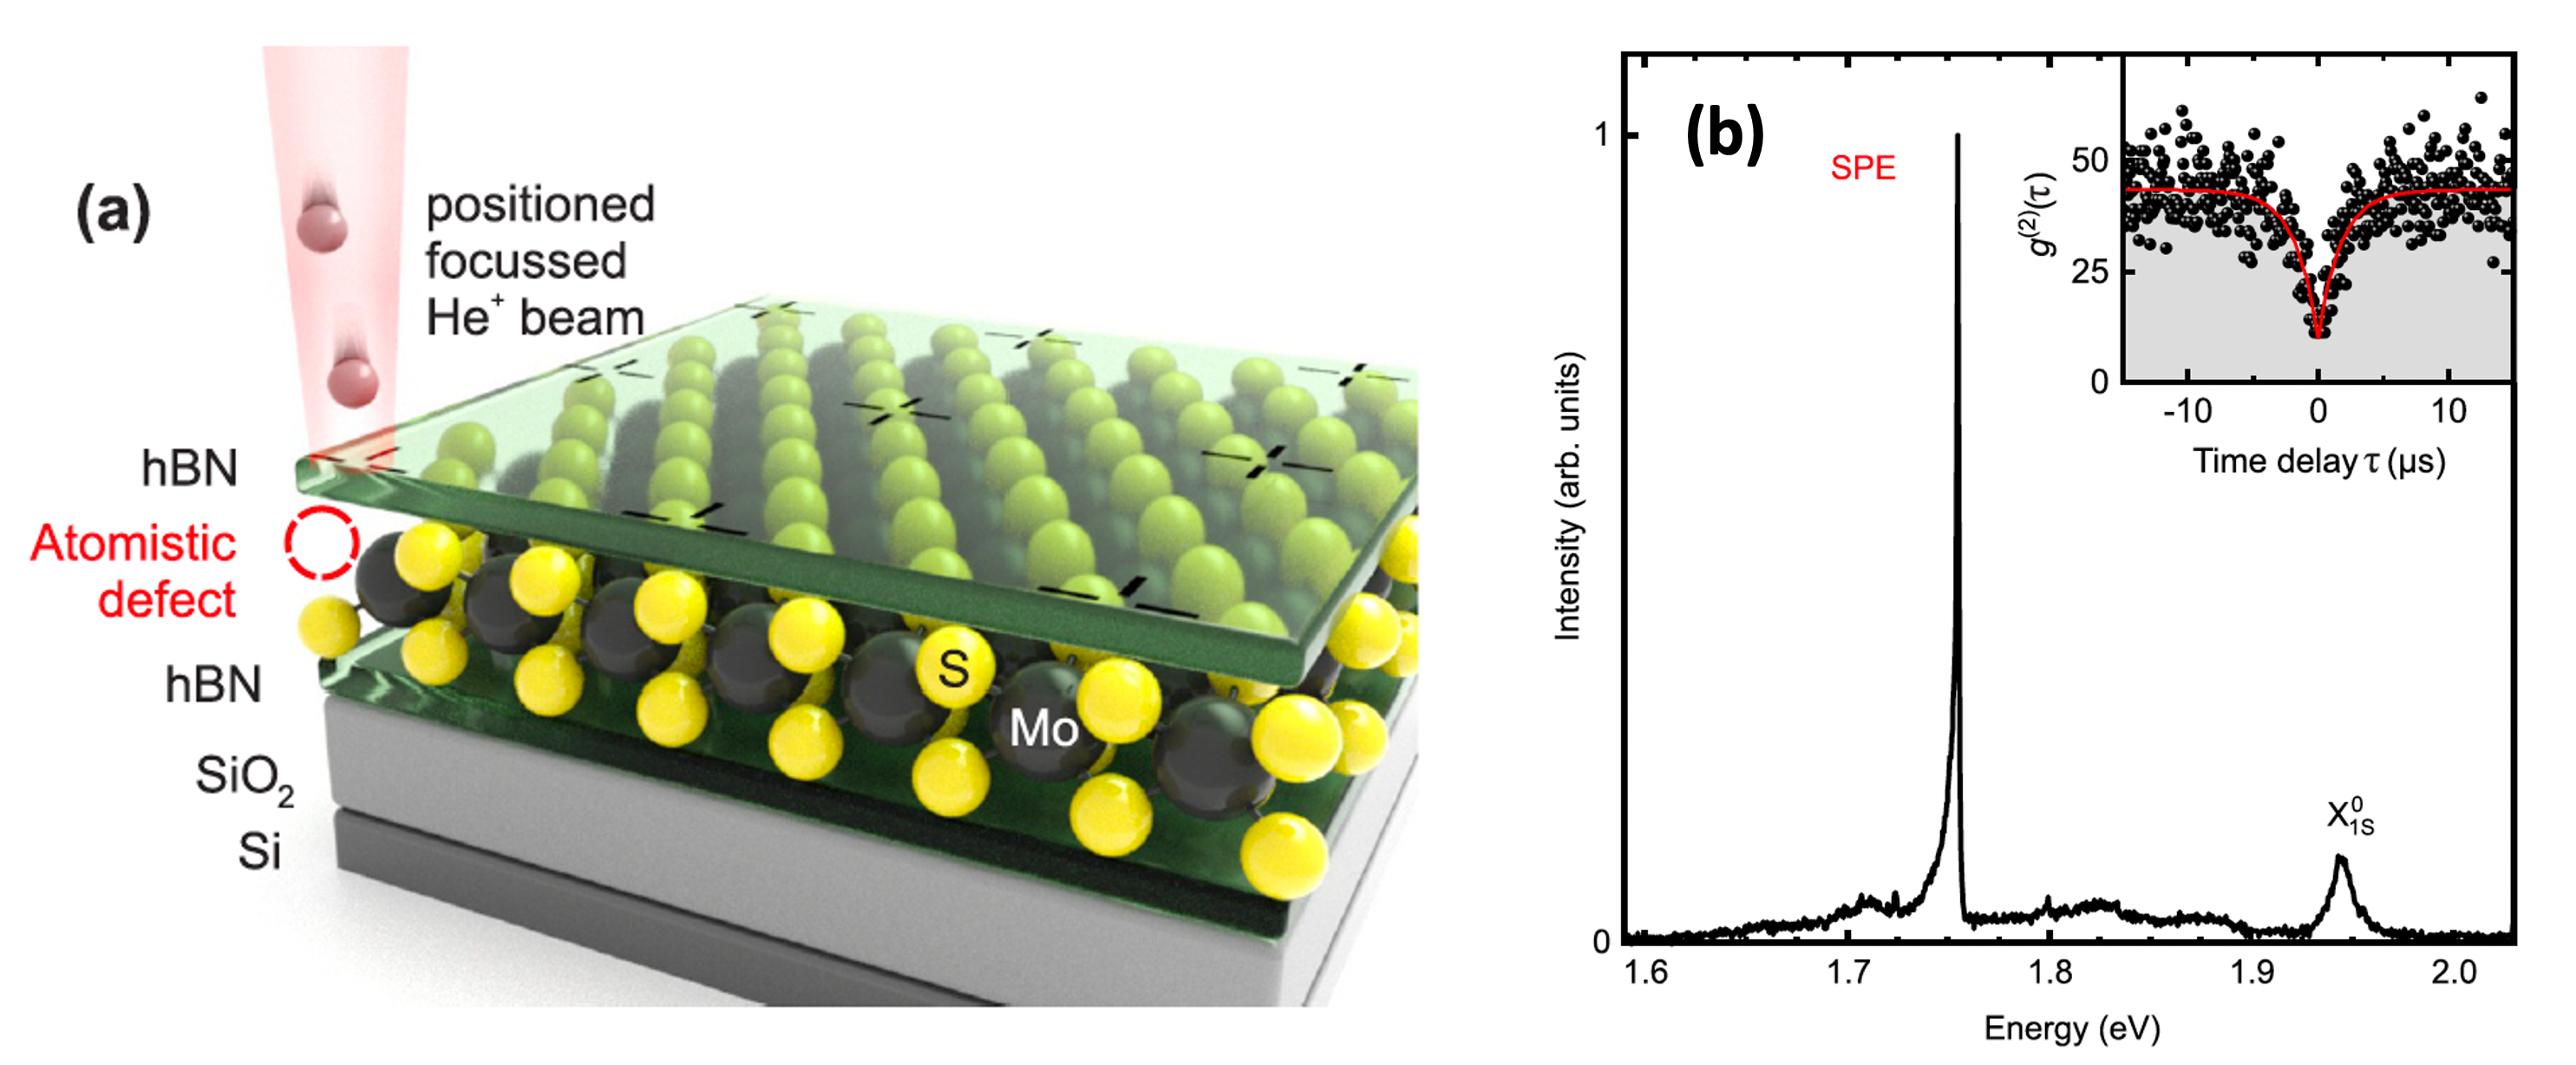
\includegraphics[width=\textwidth]{Figure/Chapter_Lipsum/single.png}
    \caption{(a) Scheme of He-ion-beam generation of sulfur vacancies in an hBN-encapsulated MoS$_2$ monolayer using a helium ion microscope (HIM). (b) Low-temperature PL spectrum showing a dominant single-photon emitter line at $\sim$1.75~eV with FWHM $\sim$28~meV, well below the MoS$_2$ exciton resonances~\cite{barthelmi2020atomistic}.}
    \label{fig:single}
    % Source: Figure/Chapter_Lipsum/single.png
    % --> Copy from /tex file/CSI 1st/images/single.png to Figure/Chapter_Lipsum/
    % Original: Barthelmi et al. APL Materials 8, 011007 (2020), Fig. 1.
\end{figure}

The characteristic spectroscopic signature of a TMD single-photon emitter comprises: (i) a spectrally isolated sharp emission line, typically 1--30~meV wide at liquid-helium temperature; (ii) a saturable emission intensity, reaching a maximum at a well-defined excitation power; (iii) a delayed onset of $\sim$100--300~ps in time-resolved PL, consistent with exciton diffusion from the generation site to the defect trapping site before radiative recombination; (iv) a single-exponential decay with a nanosecond-scale lifetime; and (v) sub-Poissonian photon statistics $g^{(2)}(0) < 0.5$ measured in the HBT configuration.

\subsubsection{Thermal Annealing as a Route to Controlled Defect Engineering}

A practical limitation of TMD-based SPEs studied so far is poor control over their spatial distribution and areal density: emitters arising from uncontrolled growth vacancies are randomly positioned, and broad-beam ion irradiation simultaneously creates a broad distribution of defect types and charge states.

Thermal annealing in vacuum offers a route to overcome these limitations.
Mitterreiter \textit{et al.}\ showed that hBN-encapsulated MoS$_2$ heated above $\sim$850~K exhibits a systematic increase in isolated single-photon emitter density with annealing temperature, consistent with thermally activated creation of sulfur vacancies~\cite{mitterreiter2021role}.
DFT calculations corroborated that the emitter binding energies and fine structure are consistent with excitons bound to sulfur mono-vacancies V$_S$.
Crucially, because the vacancy formation is thermally activated, the density of emitters can be tuned by temperature without introducing the broad lattice damage caused by ion irradiation.

% \begin{figure}[H]
%     \centering
%     % \includegraphics[width=\textwidth]{Figure/Chapter_Lipsum/thermal_annealing_SPE.png}
%     \caption{Evolution of the low-temperature PL spectrum of hBN-encapsulated MoS$_2$ as a function of annealing temperature, showing the progressive emergence of isolated single-photon emitter lines above $\sim$850~K~\cite{mitterreiter2021role}. Inset: representative $g^{(2)}(\tau)$ confirming sub-Poissonian photon statistics ($g^{(2)}(0) < 0.5$).}
%     \label{fig:thermal_SPE}
%     % Source: Mitterreiter et al. Nat. Commun. 12, 3822 (2021), Fig. 3 and Fig. 4.
% \end{figure}

The work presented in this thesis extends this thermally activated defect engineering strategy to WS$_2$, the darkish TMD with the richest low-temperature excitonic spectrum.
The combination of hBN encapsulation (for high optical quality and reduced inhomogeneous broadening), in-situ Joule heating of a suspended SiC micro-heater (for precise temperature control up to $\sim$1500~K), and low-temperature micro-photoluminescence (for spectroscopic characterisation of the resulting emitters) allows systematic investigation of thermally induced single-photon emitters in WS$_2$ with a degree of control not previously achieved.
The following chapters detail the sample fabrication, experimental methods, and spectroscopic results of this investigation.

% ---- bibliography
% \printbibheading
\printbibliography[heading=subbibintoc]
